% !TeX spellcheck = en_US
\documentclass[12pt]{article}
\usepackage{fullpage,psfrag,amsmath,amsfonts,verbatim,mathtools,scrextend}
\usepackage[small,bf]{caption}

\usepackage[framed,numbered]{mcode}

\usepackage[applemac]{inputenc}
\usepackage[T1]{fontenc}

\usepackage{url}

\usepackage[demo]{graphicx}
\usepackage{subfigure}
\usepackage{xcolor}

\usepackage{enumerate}

\bibliographystyle{alpha}

\title{Optimization and Algorithms \\ Project report}
\author{Group 42 \\ Jos{\'e} Neves 89683, Leonardo Pedroso 89691, and Gustavo Bakker 100660}
\date{}

\begin{document}
\maketitle


\section{Part 3}
In this part, the goal is to solve
\begin{equation} \label{eq:problemT4}
\begin{array}[t]{ll} 
\underset{\mathbf{y} \in \mathbf{R}^{Nk}}{\text{minimize}} & \sum_{m=1}^{N}\sum_{n=m+1}^{N}\left(||\mathbf{y_m}-\mathbf{y_n}||_2-D_{mn}\right)^2 ,\\
\end{array} 
\end{equation}
where $\mathbf{D}\in\mathbb{R}^{N\times N}$.
\subsection{Task 1}
The dataset in file \verb|data_opt.csv| is loaded and the corresponding matrix $D$ is computed according to $D_{mn} = ||\mathbf{x_m}-\mathbf{x_n}||_2$. The following MATLAB script solves task 1
\lstinputlisting{code/part3task1.m}
obtaining 
\begin{equation*}\label{key}
D_{2,3} = 5.8749, \quad D_{4,5} = 24.3769
\end{equation*} 
and 
\begin{equation*}\label{key}
\mathrm{max}(D_{mn}) = 83.003 \quad \text{for} \quad (m,n) \in \{(134,33),(33,134)\}\:.
\end{equation*}

\subsection{Task 2}
One has 
\begin{equation}\label{eq:deff}
f(\mathbf{y}) = \sum_{m=1}^{N}\sum_{n=m+1}^{N}(||\mathbf{y_m}-\mathbf{y_n}||-D_{mn})^2 = \sum_{m=1}^{N}\sum_{n=m+1}^{N} f_{mn}(\mathbf{y})^2 \:,
\end{equation}
where $\mathbf{y_m}\in \mathbb{R}^m$, $k$ is the dimension of the target space, $\mathbf{y} = \mathrm{col}(\mathbf{y_1},\ldots,\mathbf{y_N}) \in \mathbb{R}^{Nk}$ is the optimization variable, and 
\begin{equation}\label{eq:deffmn}
f_{mn}(\mathbf{y}) := ||\mathbf{y_{m-n}}||-D_{mn}\:,
\end{equation}
defining $\mathbf{y_{m-n}}$ as $\mathbf{y_{m-n}}:=\mathbf{y_m}-\mathbf{y_n}$. 

Note that one can write $\mathbf{y_m} = \mathbf{E_m}\mathbf{y}$, where $\mathbf{E_m}\in \mathbb{R}^{k\times Nk}$ is defined as 
\begin{equation*}\label{key}
\mathbf{E_m} := \left[\mathbf{0}_{k\times k(m-1)} \quad \mathbf{I}_{k\times k} \quad \mathbf{0}_{k\times k(N-m)}  \right]\:, 
\end{equation*}
thus, it is possible to rewrite \eqref{eq:deffmn} as
\begin{equation}\label{eq:deffmnnew}
f_{mn}(\mathbf{y}) = ||\mathbf{E_m}\mathbf{y}-\mathbf{E_n}\mathbf{y}||-D_{mn} = \sqrt{\mathbf{y}^T(\mathbf{E_m}-\mathbf{E_n})^T(\mathbf{E_m}-\mathbf{E_n})\mathbf{y}}-D_{mn}\:.
\end{equation}
Taking the jacobian of \eqref{eq:deffmnnew}, one obtains
\begin{equation}\label{eq:gradfmn}
\begin{split}
D_{\mathbf{y}}f_{m,n}(\mathbf{y}) &= D_u(\sqrt{u})\biggr\rvert_{u = \mathbf{y}^T(\mathbf{E_m}-\mathbf{E_n})^T(\mathbf{E_m}-\mathbf{E_n})\mathbf{y}}D_{\mathbf{y}}(\mathbf{y}^T(\mathbf{E_m}-\mathbf{E_n})^T(\mathbf{E_m}-\mathbf{E_n})\mathbf{y})\\
&= \mathbf{y}^T\frac{(\mathbf{E_m}-\mathbf{E_n})^T(\mathbf{E_m}-\mathbf{E_n})}{\sqrt{\mathbf{y}^T(\mathbf{E_m}-\mathbf{E_n})^T(\mathbf{E_m}-\mathbf{E_n})\mathbf{y}}}\\
&=\frac{\left[\mathbf{0}_{1\times(m-1)k} \quad  \mathbf{y_{m-n}}^T \quad \mathbf{0}_{1\times(n-m-1)k} \quad -\mathbf{y_{m-n}}^T \quad \mathbf{0}_{1\times(N-n)k}  \right]}{||\mathbf{y_{m-n}}||}
\end{split}
\end{equation}
therefore the gradient $\nabla_{\mathbf{y}} f_{mn}(\mathbf{y}) = \left(D_{\mathbf{y}}f_{mn}(\mathbf{y})\right)^T$.

\begin{comment}
is given by
\begin{equation}\label{eq:gradfmn}
\nabla_{\mathbf{y}} f_{mn}(\mathbf{y}) =  \frac{(\mathbf{E_m}-\mathbf{E_n})^T(\mathbf{E_m}-\mathbf{E_n})}{f_{mn}(\mathbf{y})+D_{mn}} \mathbf{y}\:.
\end{equation}
\end{comment}


Similarly taking the jacobian of \eqref{eq:deff}, one obtains
\begin{equation*}\label{key}
D_{\mathbf{y}}f(\mathbf{y}) = \sum_{m=1}^{N}\sum_{n=m+1}^{N} D_u(u^2)\biggr\rvert_{u=f_{mn}(\mathbf{y})}D_{\mathbf{y}}f_{mn}(\mathbf{y})\\= \sum_{m=1}^{N}\sum_{n=m+1}^{N} 2f_{mn}(\mathbf{y})D_{\mathbf{y}}f_{mn}(\mathbf{y})
\end{equation*}
therefore the gradient $\nabla_{\mathbf{y}} f(\mathbf{y}) = \left(D_{\mathbf{y}}f(\mathbf{y})\right)^T$ is given by
\begin{equation}\label{eq:gradf}
\nabla_{\mathbf{y}} f(\mathbf{y}) = \sum_{m=1}^{N}\sum_{n=m+1}^{N} 2f_{mn}(\mathbf{y})\nabla_{\mathbf{y}}f_{mn}(\mathbf{y})
\end{equation}
In conclusion, $f(\mathbf{y})$, $f_{mn}(\mathbf{y})$,$\nabla_{\mathbf{y}} f_{mn}(\mathbf{y})$, and $\nabla_{\mathbf{y}} f(\mathbf{y})$ can be computed making use of \eqref{eq:deff},\eqref{eq:deffmn}, \eqref{eq:gradfmn}, and \eqref{eq:gradf}, respectively. Also note that each of these four quantities may be computed making use of differences of the optimization vector exclusively, \textit{i.e.}, the $N(N/2-1)$ vectors $\mathbf{y_{m-n}}$. As it is explored herein this property allows for considerable optimization of the computational load required to solve the optimization problem.

For the implementation of the Levenberg-Marquardt (LM) method is is required to compute, for each new iteration, $f(\mathbf{y})$, $||\nabla_{\mathbf{y}} f(\mathbf{y})||$, matrix $\mathbf{A}$, and vector $\mathbf{b}$, defined by
\begin{equation}\label{eq:matAb}
\mathbf{A}:= \begin{bmatrix}
D_{\mathbf{y}} f_{1,1}(\mathbf{y})\\
D_{\mathbf{y}} f_{1,2}(\mathbf{y})\\\vdots\\
D_{\mathbf{y}} f_{N-1,N}(\mathbf{y})\\
\sqrt{\lambda}\mathbf{I}_{Nk\times Nk}
\end{bmatrix}\quad \text{and} \quad \mathbf{b}:= \begin{bmatrix}
D_{\mathbf{y}} f_{1,1}(\mathbf{y})\mathbf{y}-f_{1,1}(\mathbf{y})\\
D_{\mathbf{y}} f_{1,2}(\mathbf{y})\mathbf{y}-f_{1,2}(\mathbf{y})\\\vdots\\
D_{\mathbf{y}} f_{N-1,N}(\mathbf{y})\mathbf{y}-f_{N-1,N}(\mathbf{y})\\
\sqrt{\lambda}\mathbf{y}
\end{bmatrix}\:.
\end{equation}
For that purpose a MATLAB function independent of the LM algorithm is devised. This allows to implement the LM algorithm separately, which can then be applied to any optimization problem of suitable form, and not being constrained to the problem at hand in this part. To allow for a computationally efficient algorithm to compute, at each iteration, the relevant quantities related to the objective function, first note that 
\begin{equation}\label{eq:matAbsimp}
D_{\mathbf{y}} f_{mn}(\mathbf{y})\mathbf{y}-f_{mn}(\mathbf{y}) = \frac{\mathbf{y_{m-n}}(\mathbf{y_m}-\mathbf{y_n})}{||\mathbf{y_{m-n}}||}-||\mathbf{y_{m-n}}||+D_{mn} = D_{mn}\:.
\end{equation}
Thus, noticing that $\mathbf{b}$ in \eqref{eq:matAb} results of the concatenation of terms of the form \eqref{eq:matAbsimp}, $\mathbf{b}$ is computed according to
\begin{equation}\label{eq:b}
\mathbf{b}= \left[D_{1,1}\;\;\;\;D_{1,2}\;\;\;\;\ldots \;\;\;\;D_{N-1,N}\;\;\;\; \sqrt{\lambda}\mathbf{y} \right]\:,
\end{equation}
which is very efficiently computed since it does not have to carried out iteratively. Furthermore, a significant portion of $\mathbf{b}$ is constant, which has to be computed just once in the LM algorithm. Second, the computation of $f(\mathbf{y})$, $||\nabla_{\mathbf{y}} f(\mathbf{y})||$, and $\mathbf{A}$ is performed iteratively, running one iteration for each of the $N(N/2-1)$ vectors $\mathbf{y_{m-n}}$. Therefore, it is more efficient to compute all of these quantities at once. Third, $\lambda$ is a variable of the LM method, which does not depend directly on the objective function, thus, it was chosen that the entries of $\mathbf{A}$ and $\mathbf{b}$ which are dependent on $\lambda$ are computed in the LM algorithm function. Fourth, an effort was made so that there is not replication of computations. Given that, the quantities computed depend essentially on each other, $\mathbf{y_{m-n}}$, or $||\mathbf{y_{m-n}}||$, then this allows to reduce the computational load significantly.

Having the aforementioned optimization guidelines in mind the following MATLAB function was designed
\lstinputlisting{code/objectiveF.m}
This implementation allows for a decrease of computation time of roughly two orders of magnitude compared with a first naive implementation.

\subsection{Task 3}
In this task the optimization problem is solved for the dataset loaded in Task 1, for $k \in \{2,3\}$, using the LM algorithm. For that reason, a generic implementation of this algorithm was implemented in MATLAB
\lstinputlisting{code/LMAlgorithm.m}
Note that this implementation relies on the fact that $f(\mathbf{y})$, $||\nabla_{\mathbf{y}} f(\mathbf{y})||$, matrix $\mathbf{A}$, and vector $\mathbf{b}$ are computed at once. It is important to remark, however, that each time a step is invalid, the new $\mathbf{A}$ and $\mathbf{b}$ that were computed are useless, which represents a waste of computational power. It was verified that, for this particular optimization problem, reduction that is achieved computing all quantities at once is greater than that obtained if $\mathbf{A}$ and $\mathbf{b}$ are only computed when necessary.

The following MATLAB script was then run to solve the optimization problem 
\lstinputlisting{code/part3task3.m}.

The results obtained for $k=2$ are shown in Figs. \ref{fig:task3_LM_k_2} and \ref{fig:task3_lowerDim_k_2}, and for $k=3$ in Figs. \ref{fig:task3_LM_k_3} and \ref{fig:task3_lowerDim_k_3}.

\begin{figure}[ht]
	\centering
	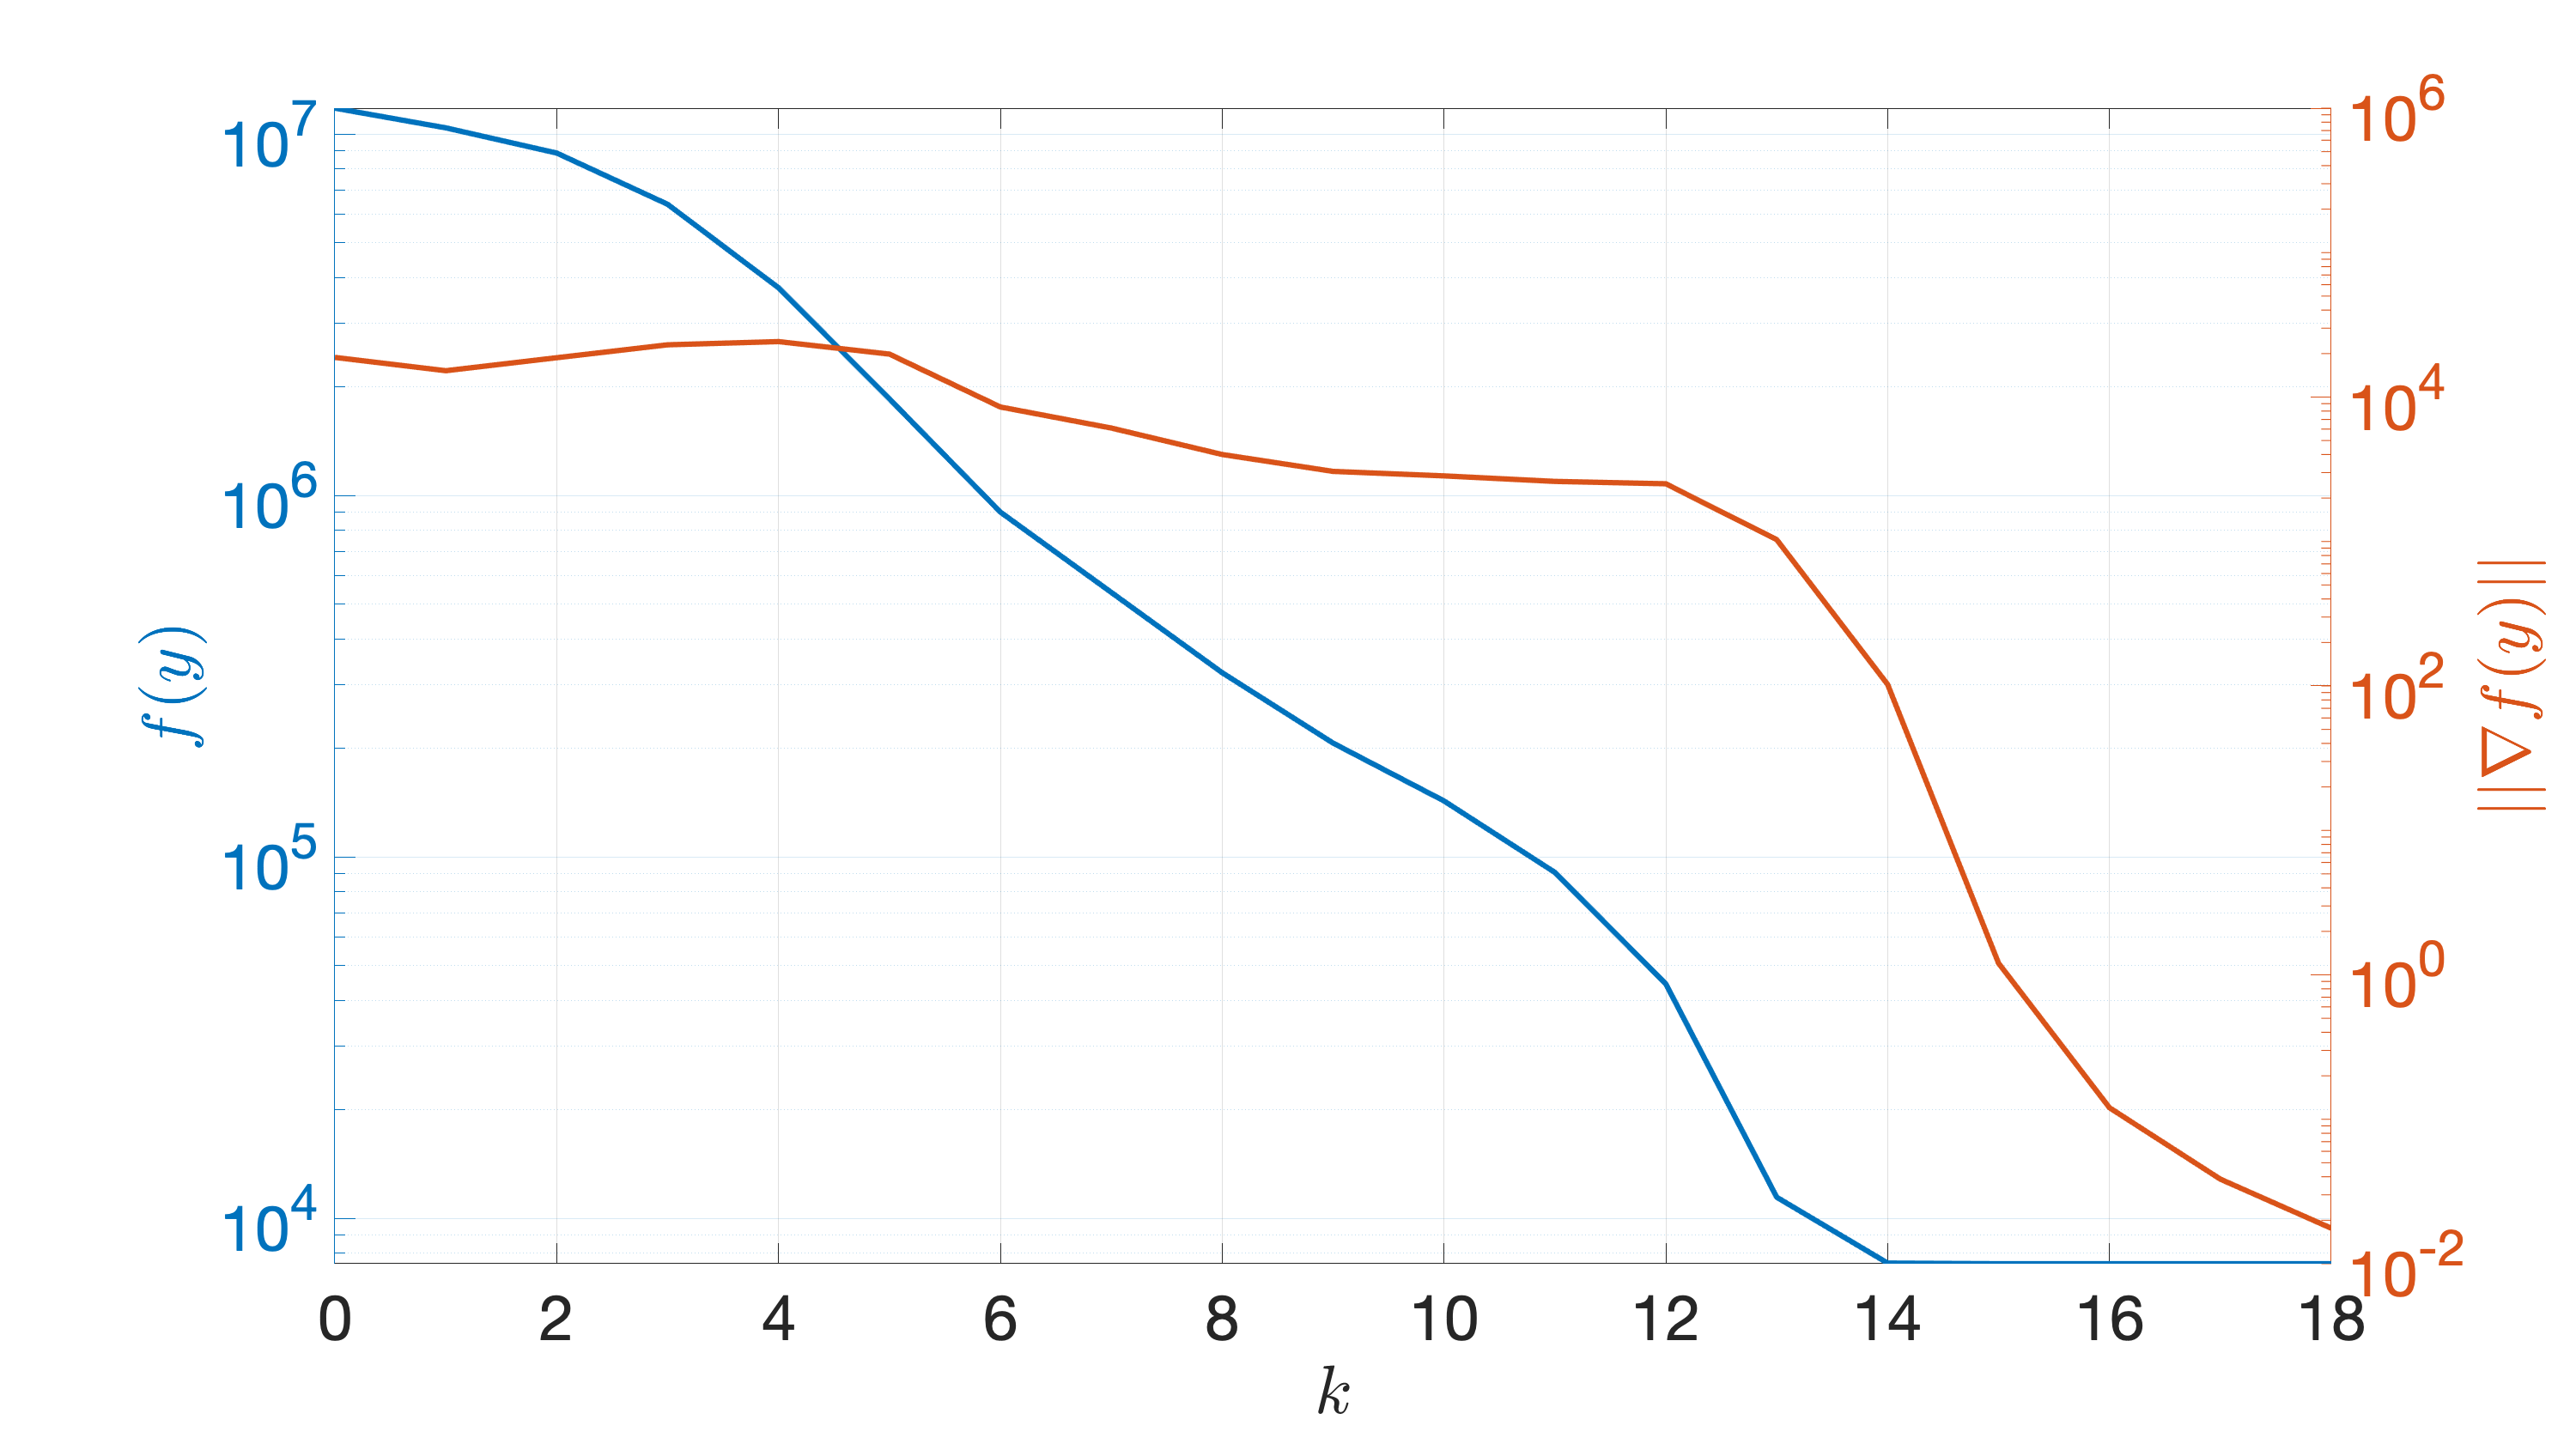
\includegraphics[width=0.9\textwidth]{figures/task3_LM_k_2.png}
	\caption{Objective function value and gradient norm throughout the iterations of the LM algorithm for $k=2$.}
	\label{fig:task3_LM_k_2}
\end{figure}

\begin{figure}[h!]
	\centering
	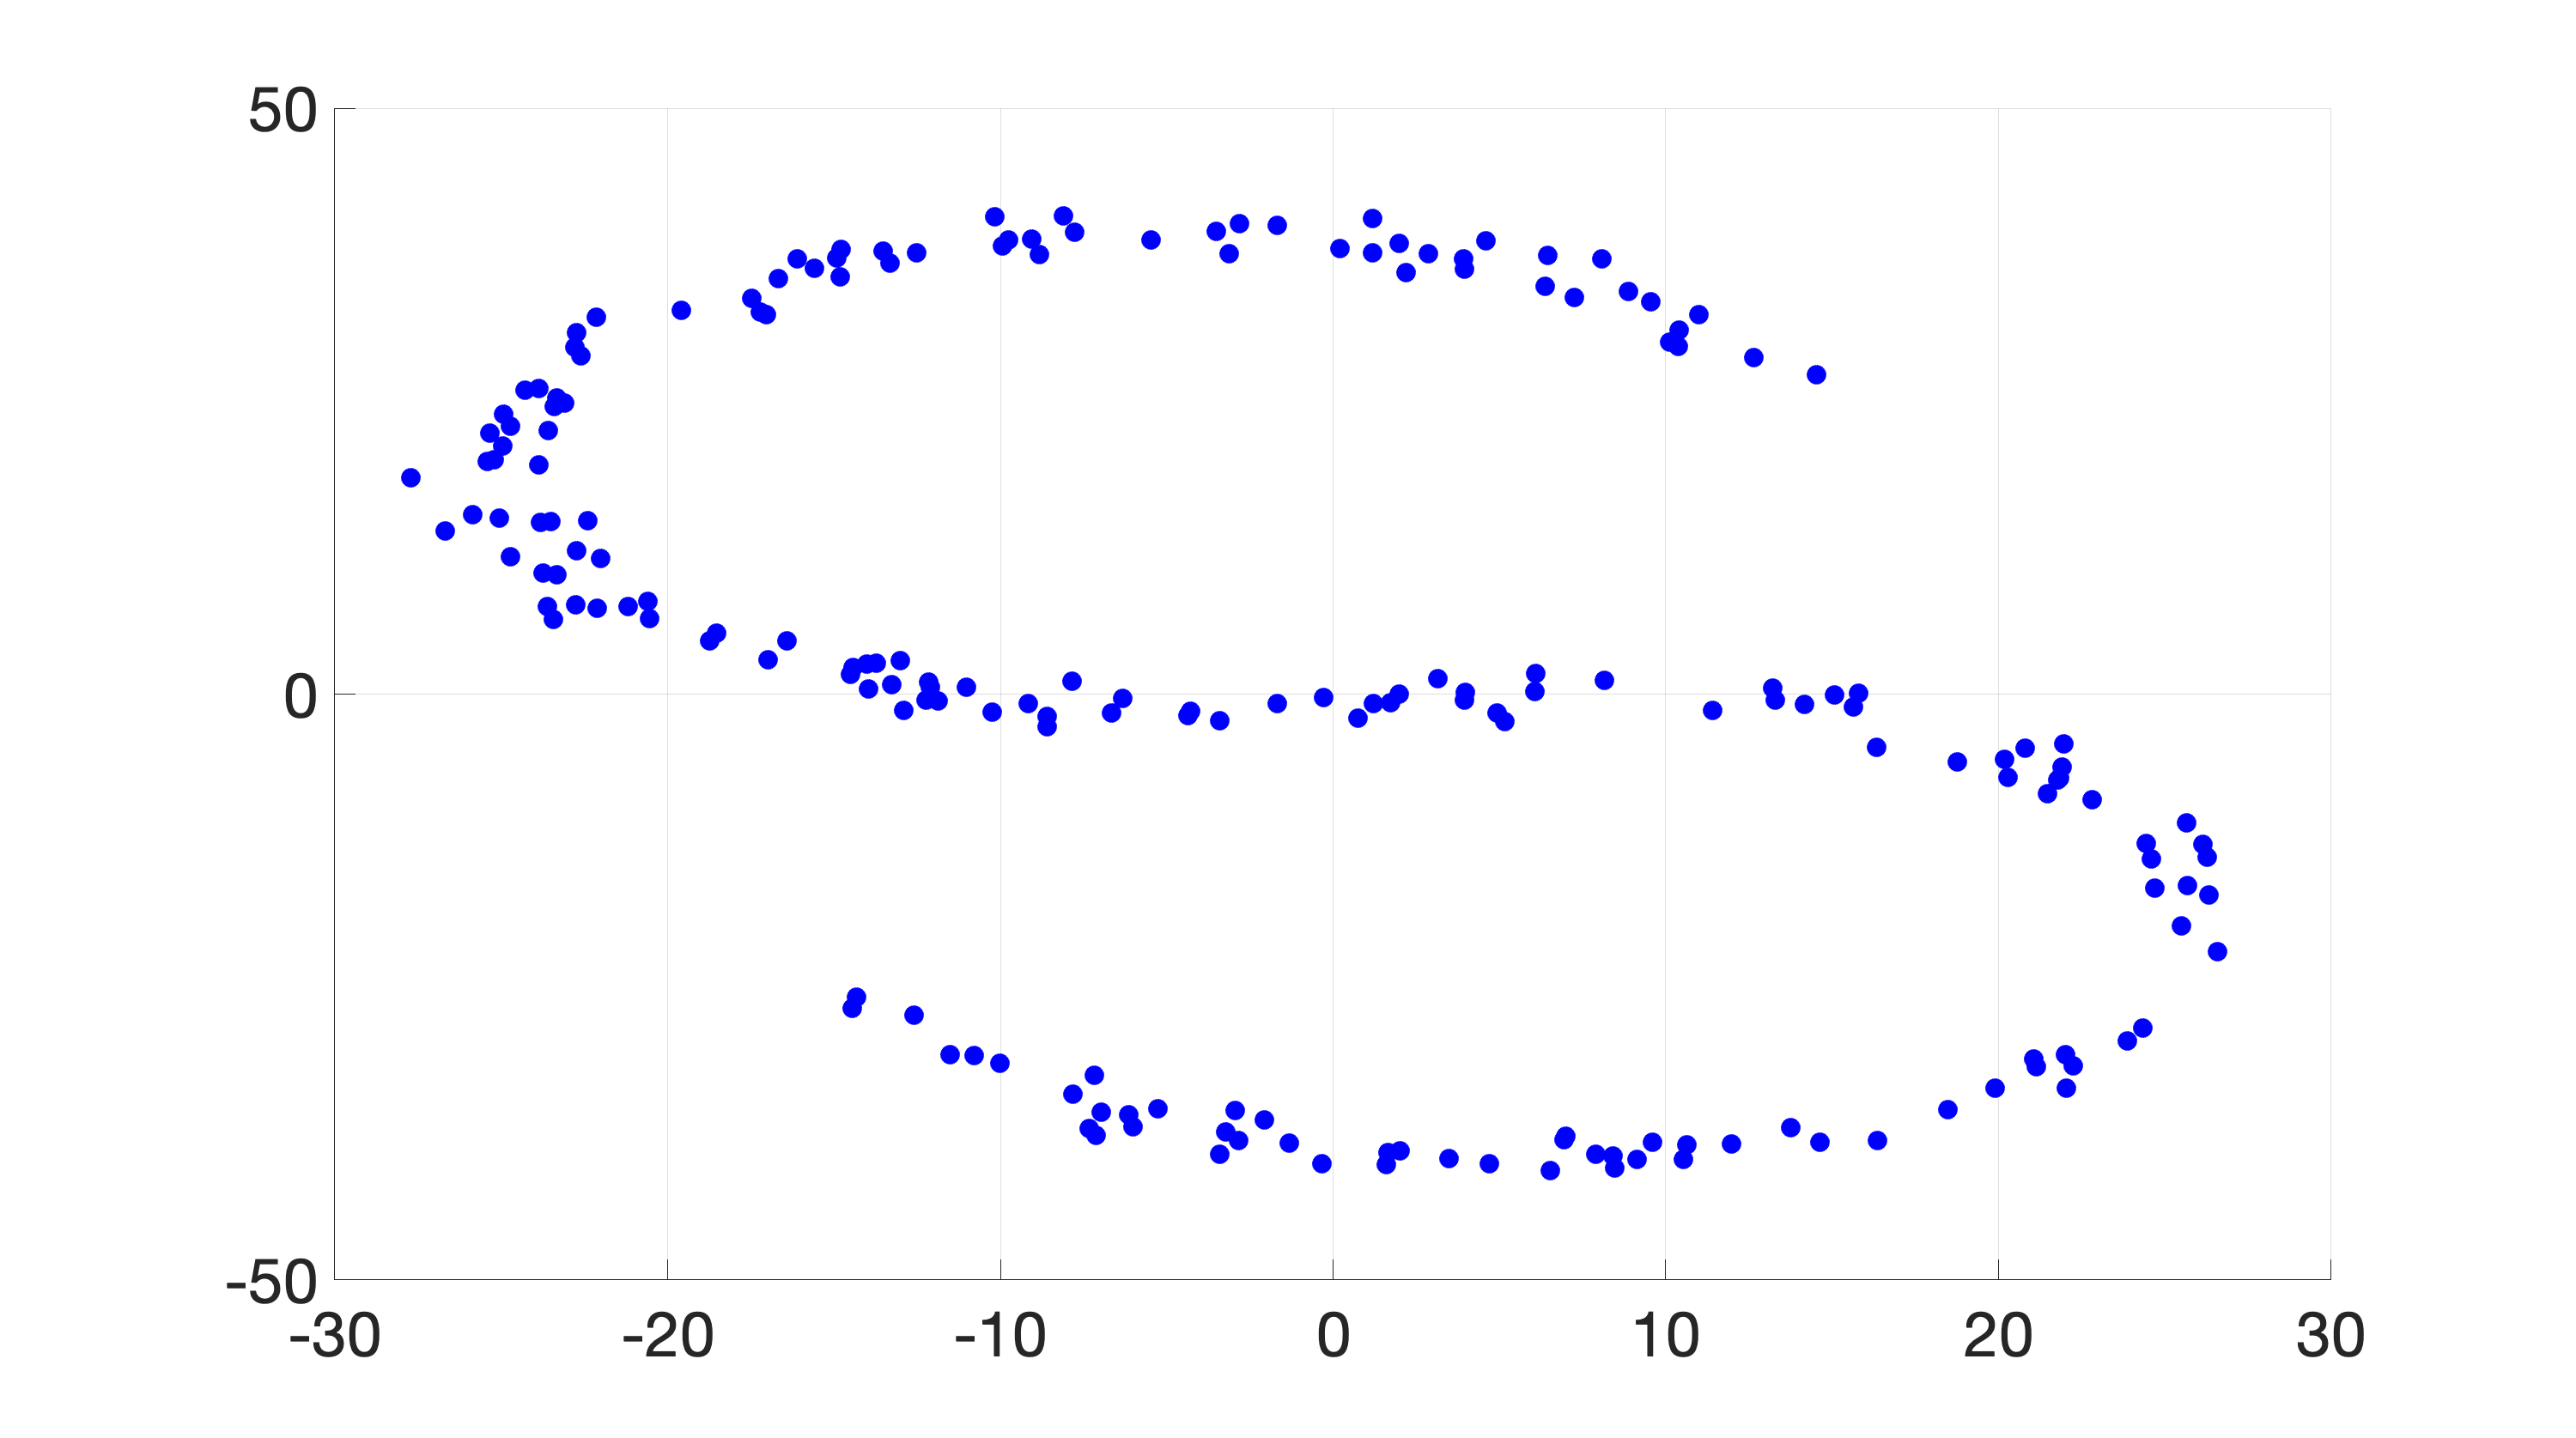
\includegraphics[width=0.9\textwidth]{figures/task3_lowerDim_k_2.png}
	\caption{Solution to the optimization problem using the LM algorithm for $k=2$.}
	\label{fig:task3_lowerDim_k_2}
\end{figure}

\begin{figure}[ht!]
	\centering
	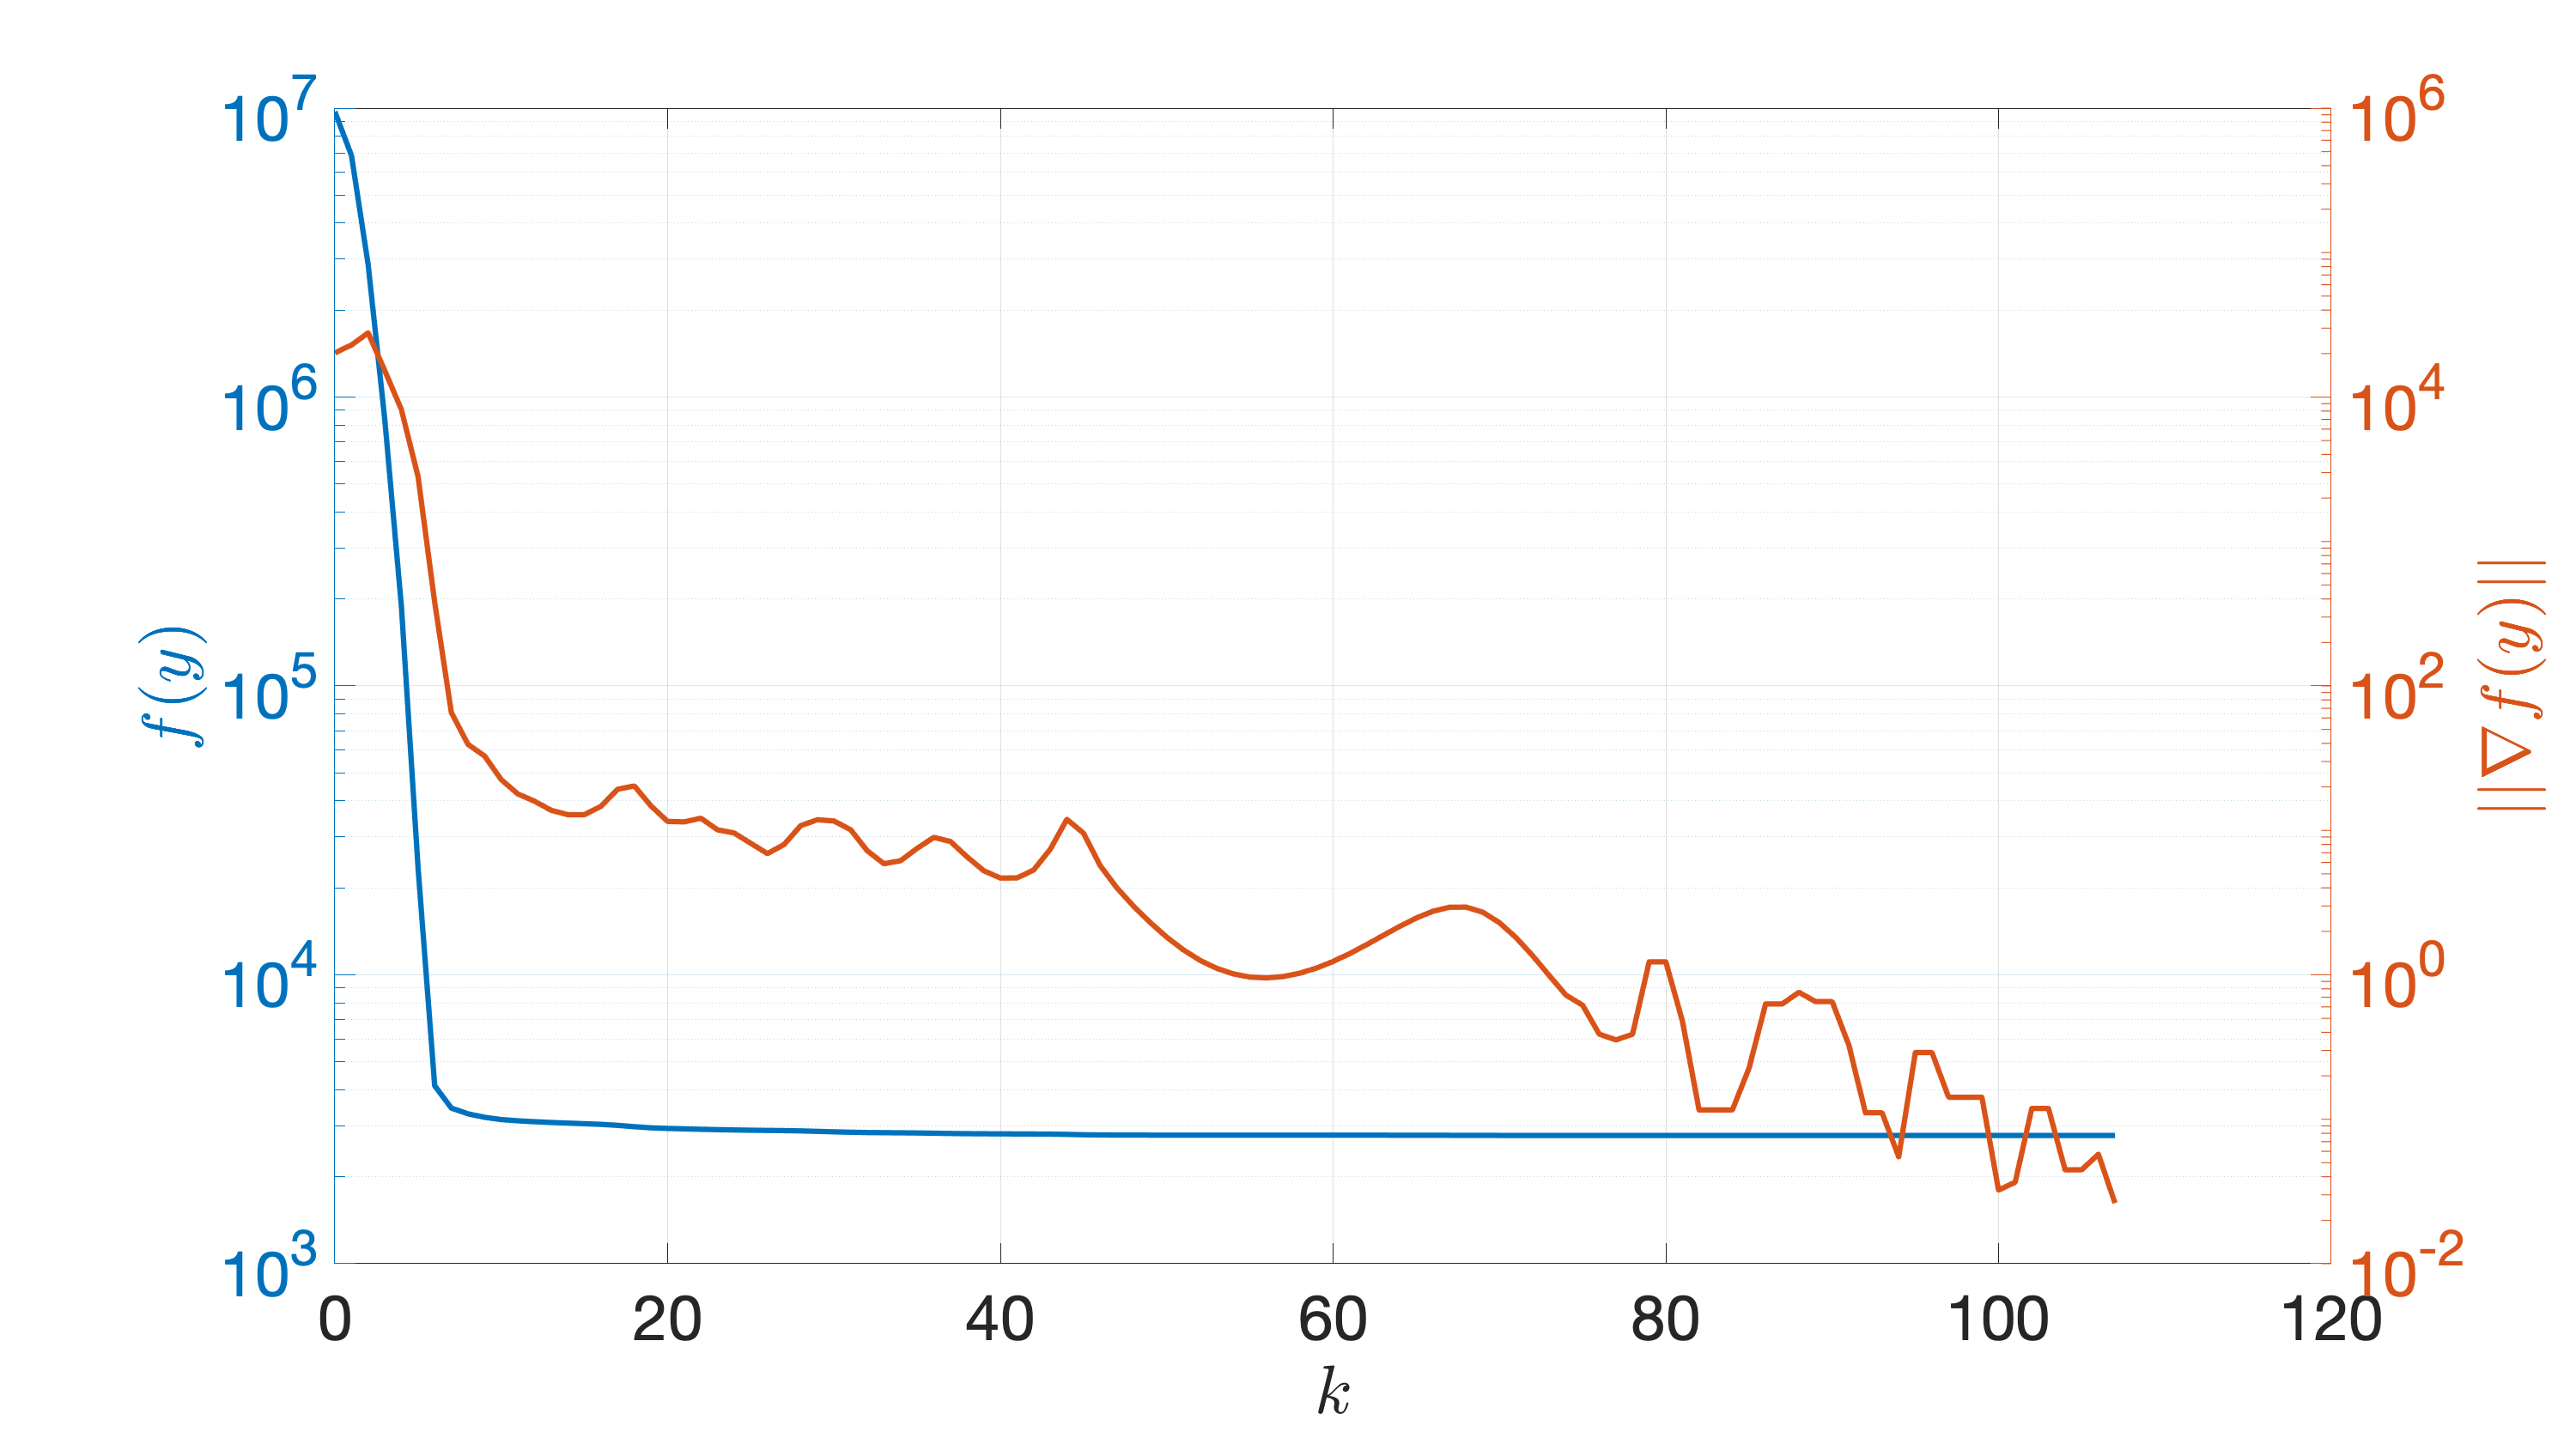
\includegraphics[width=0.9\textwidth]{figures/task3_LM_k_3.png}
	\caption{Objective function value and gradient norm throughout the iterations of the LM algorithm for $k=2$.}
	\label{fig:task3_LM_k_3}
\end{figure}

\begin{figure}[ht!]
	\centering
	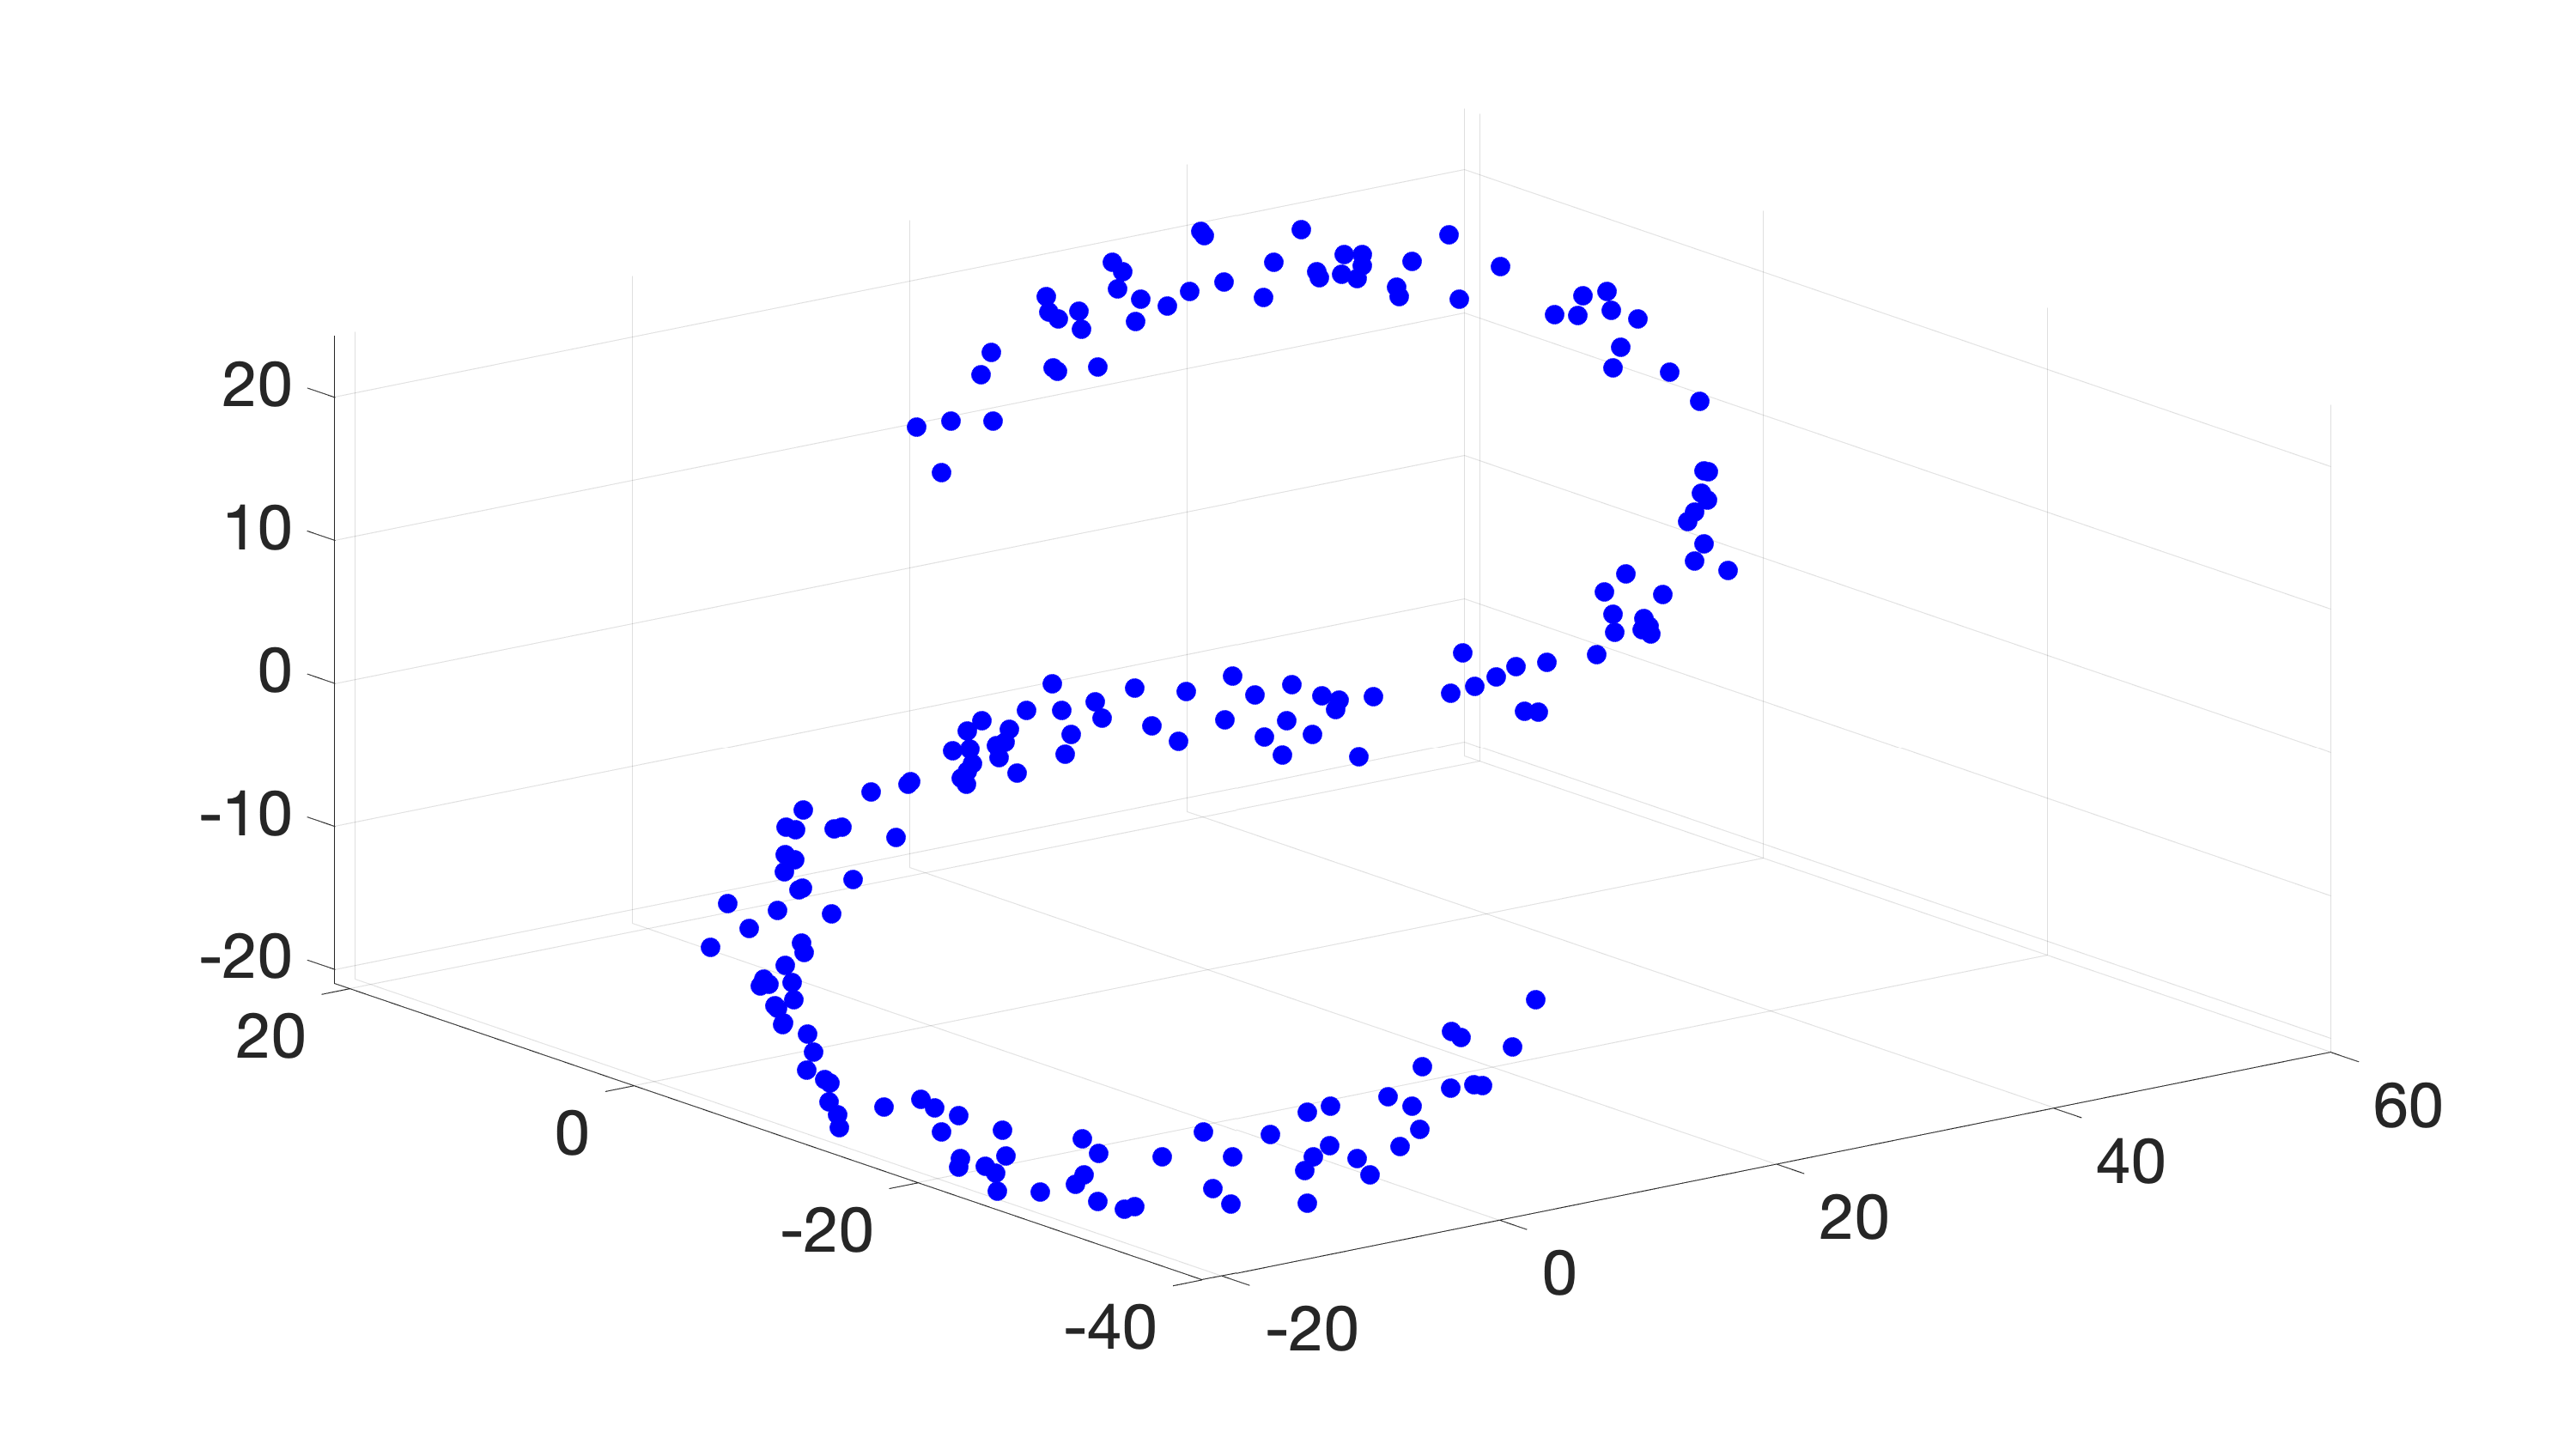
\includegraphics[width=0.9\textwidth]{figures/task3_lowerDim_k_3.png}
	\caption{Solution to the optimization problem using the LM algorithm for $k=2$.}
	\label{fig:task3_lowerDim_k_3}
\end{figure}

First, it is noticeable that the algorithm converges and reaches the expected solution for both values of $k$. Second, the value of the objective function of both solutions is shown in Table \ref{tb:costFunction}. It is visible that the value of the cost function for $k=3$ decreases by a factor of roughly $2.7$ in relation to the solution with $k=2$. Thus, $k=3$ fits much better to the dataset. Third, note that the solution using $k=3$ requires more iterations of the LM algorithm than what is presented in the provided results. In fact, observing the evolution of the norm of the gradient of the objective function, visible in Fig. \ref{fig:task3_LM_k_3}, it is possible to detect the presence of numerical error stating at the 70-th iteration, which arises using MATLAB 2018a. For this reason, although the solution is identical, it takes more iterations to reach the stopping criterion. 

\begin{table}[ht!]
	\centering
	\caption{Value of the objective function of both solutions.}
	\label{tb:costFunction}
	\begin{tabular}{c c c}
		\hline
		$k$&$\quad$ & $f(\mathbf{y})$\\ \hline
		2 &$\quad$ & 7486.6\\
		3 &$\quad$ & 2779.2\\
		\hline
	\end{tabular}
\end{table} 

\subsection{Task 4}
The LM method is now applied to dataset\verb|dataProj.csv|, and we are not provided with an initialization $\mathbf{y}_0$. There is no guarantee that a solution found by the LM method is the global solution, since the objective function is not convex. For this reason, to find a good suboptimal solution, the method has to be run several times for different randomly generated initializations. The solutions are then sorted according to the value of the objective function, of which the best is chosen. It is very important to remark that the computation of each of the solutions can be run in a parallel manner, using the \textit{Parallel toolbox} in MATLAB, for instance. The following MATLAB script solves task 4.
\lstinputlisting{code/part3task4.m}.

The LM algorithm was run for 24 different randomly generated initialization vectors, in a parallel manner. The best solution, obtained for $k=2$, is shown in Figs. \ref{fig:task4_LM} and \ref{fig:task4_sol}, achieving an objective function value of $f(\mathbf{y}_{sol}) = 7.6430\times 10^{-5}$. First, the parallel computation of the various solutions allowed for a significantly faster computation. Second, it was verified that all solutions obtained have identical objective function values, which on its own does not imply that it is the global solution. Notice that the objective function is nonnegative. Furthermore, it is verified that if the stopping criteria parameter is lowered then this method yields an objective function value that it closer to zero. For this reason, as the order of magnitude of the entries of $D$ is substantially greater than the order of magnitude of the objective function value at the solutions, either the problem is ill-conditioned or one of the global minimums (or the only global minimum) was found. Assuming the problem is not ill-conditioned, then, even though this claim is not theoretically correct, it is possible to assume in a practical sense that one approximation very close the global minimizer was found. 
\begin{figure}[ht!]
	\centering
	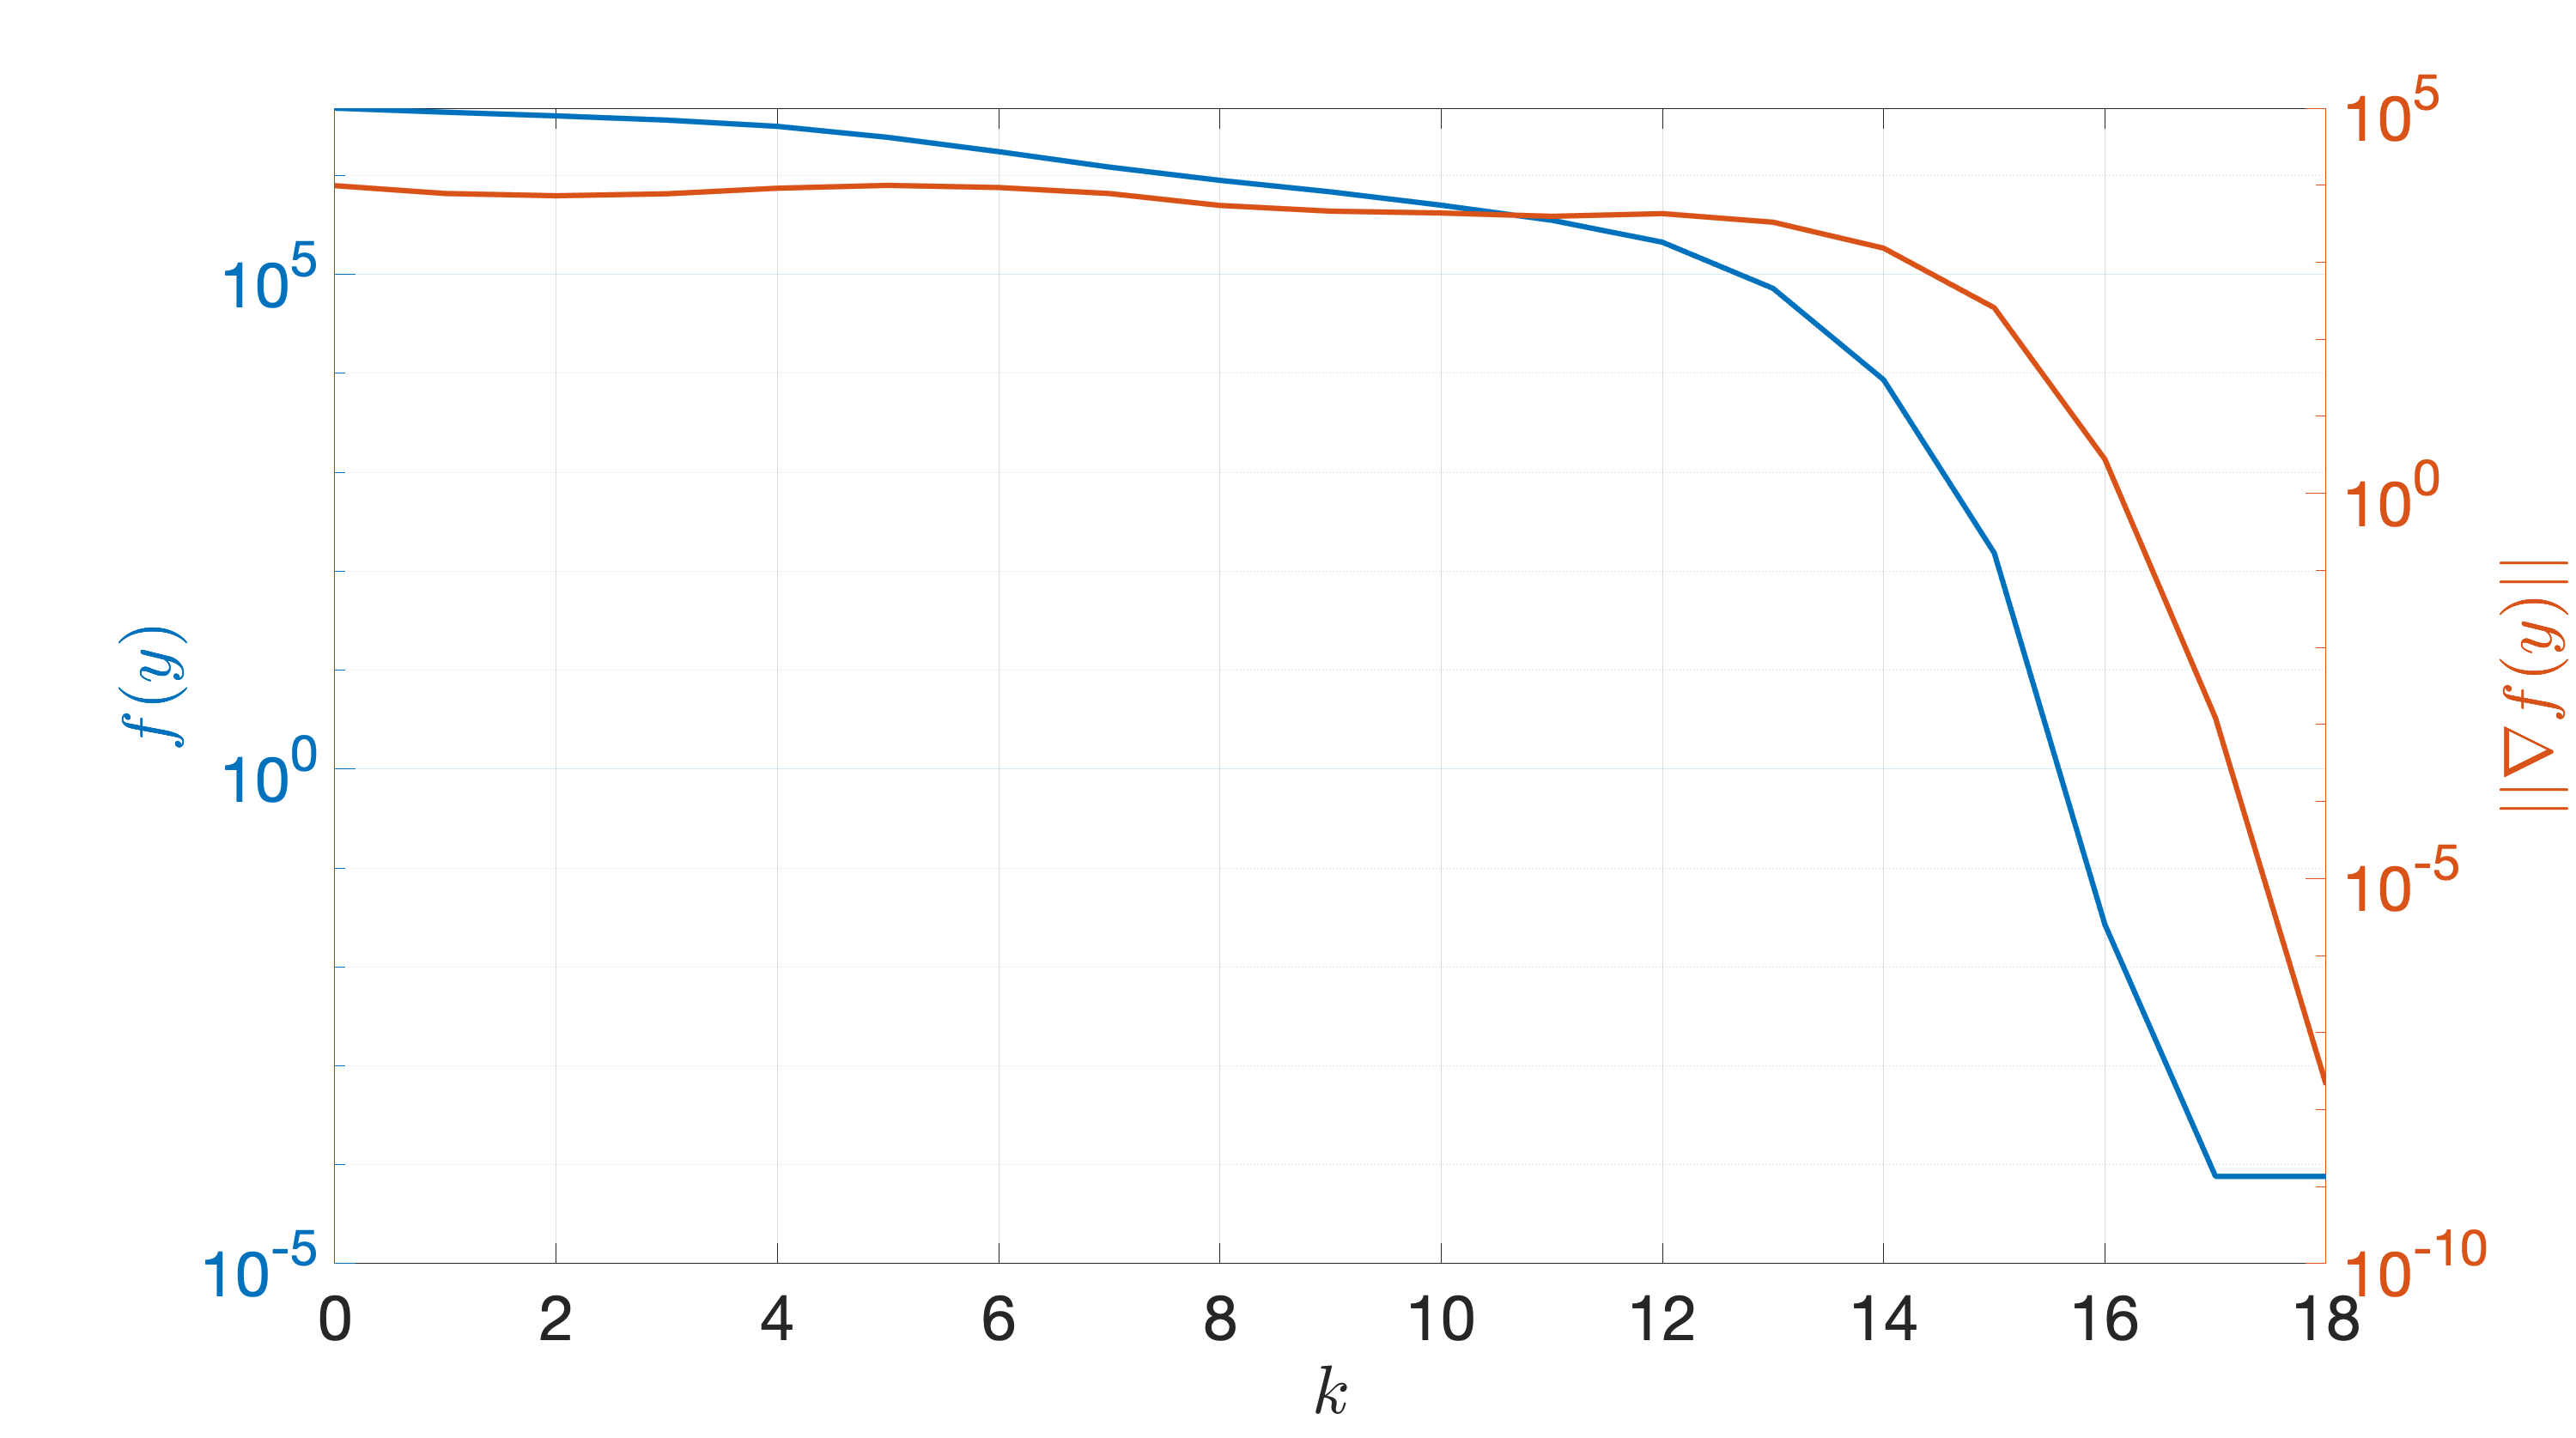
\includegraphics[width=0.9\textwidth]{figures/task4_LM.png}
	\caption{Objective function value and gradient norm throughout the iterations of the LM algorithm for the dataset of task 4 and $k=2$.}
	\label{fig:task4_LM}
\end{figure}

\begin{figure}[ht!]
	\centering
	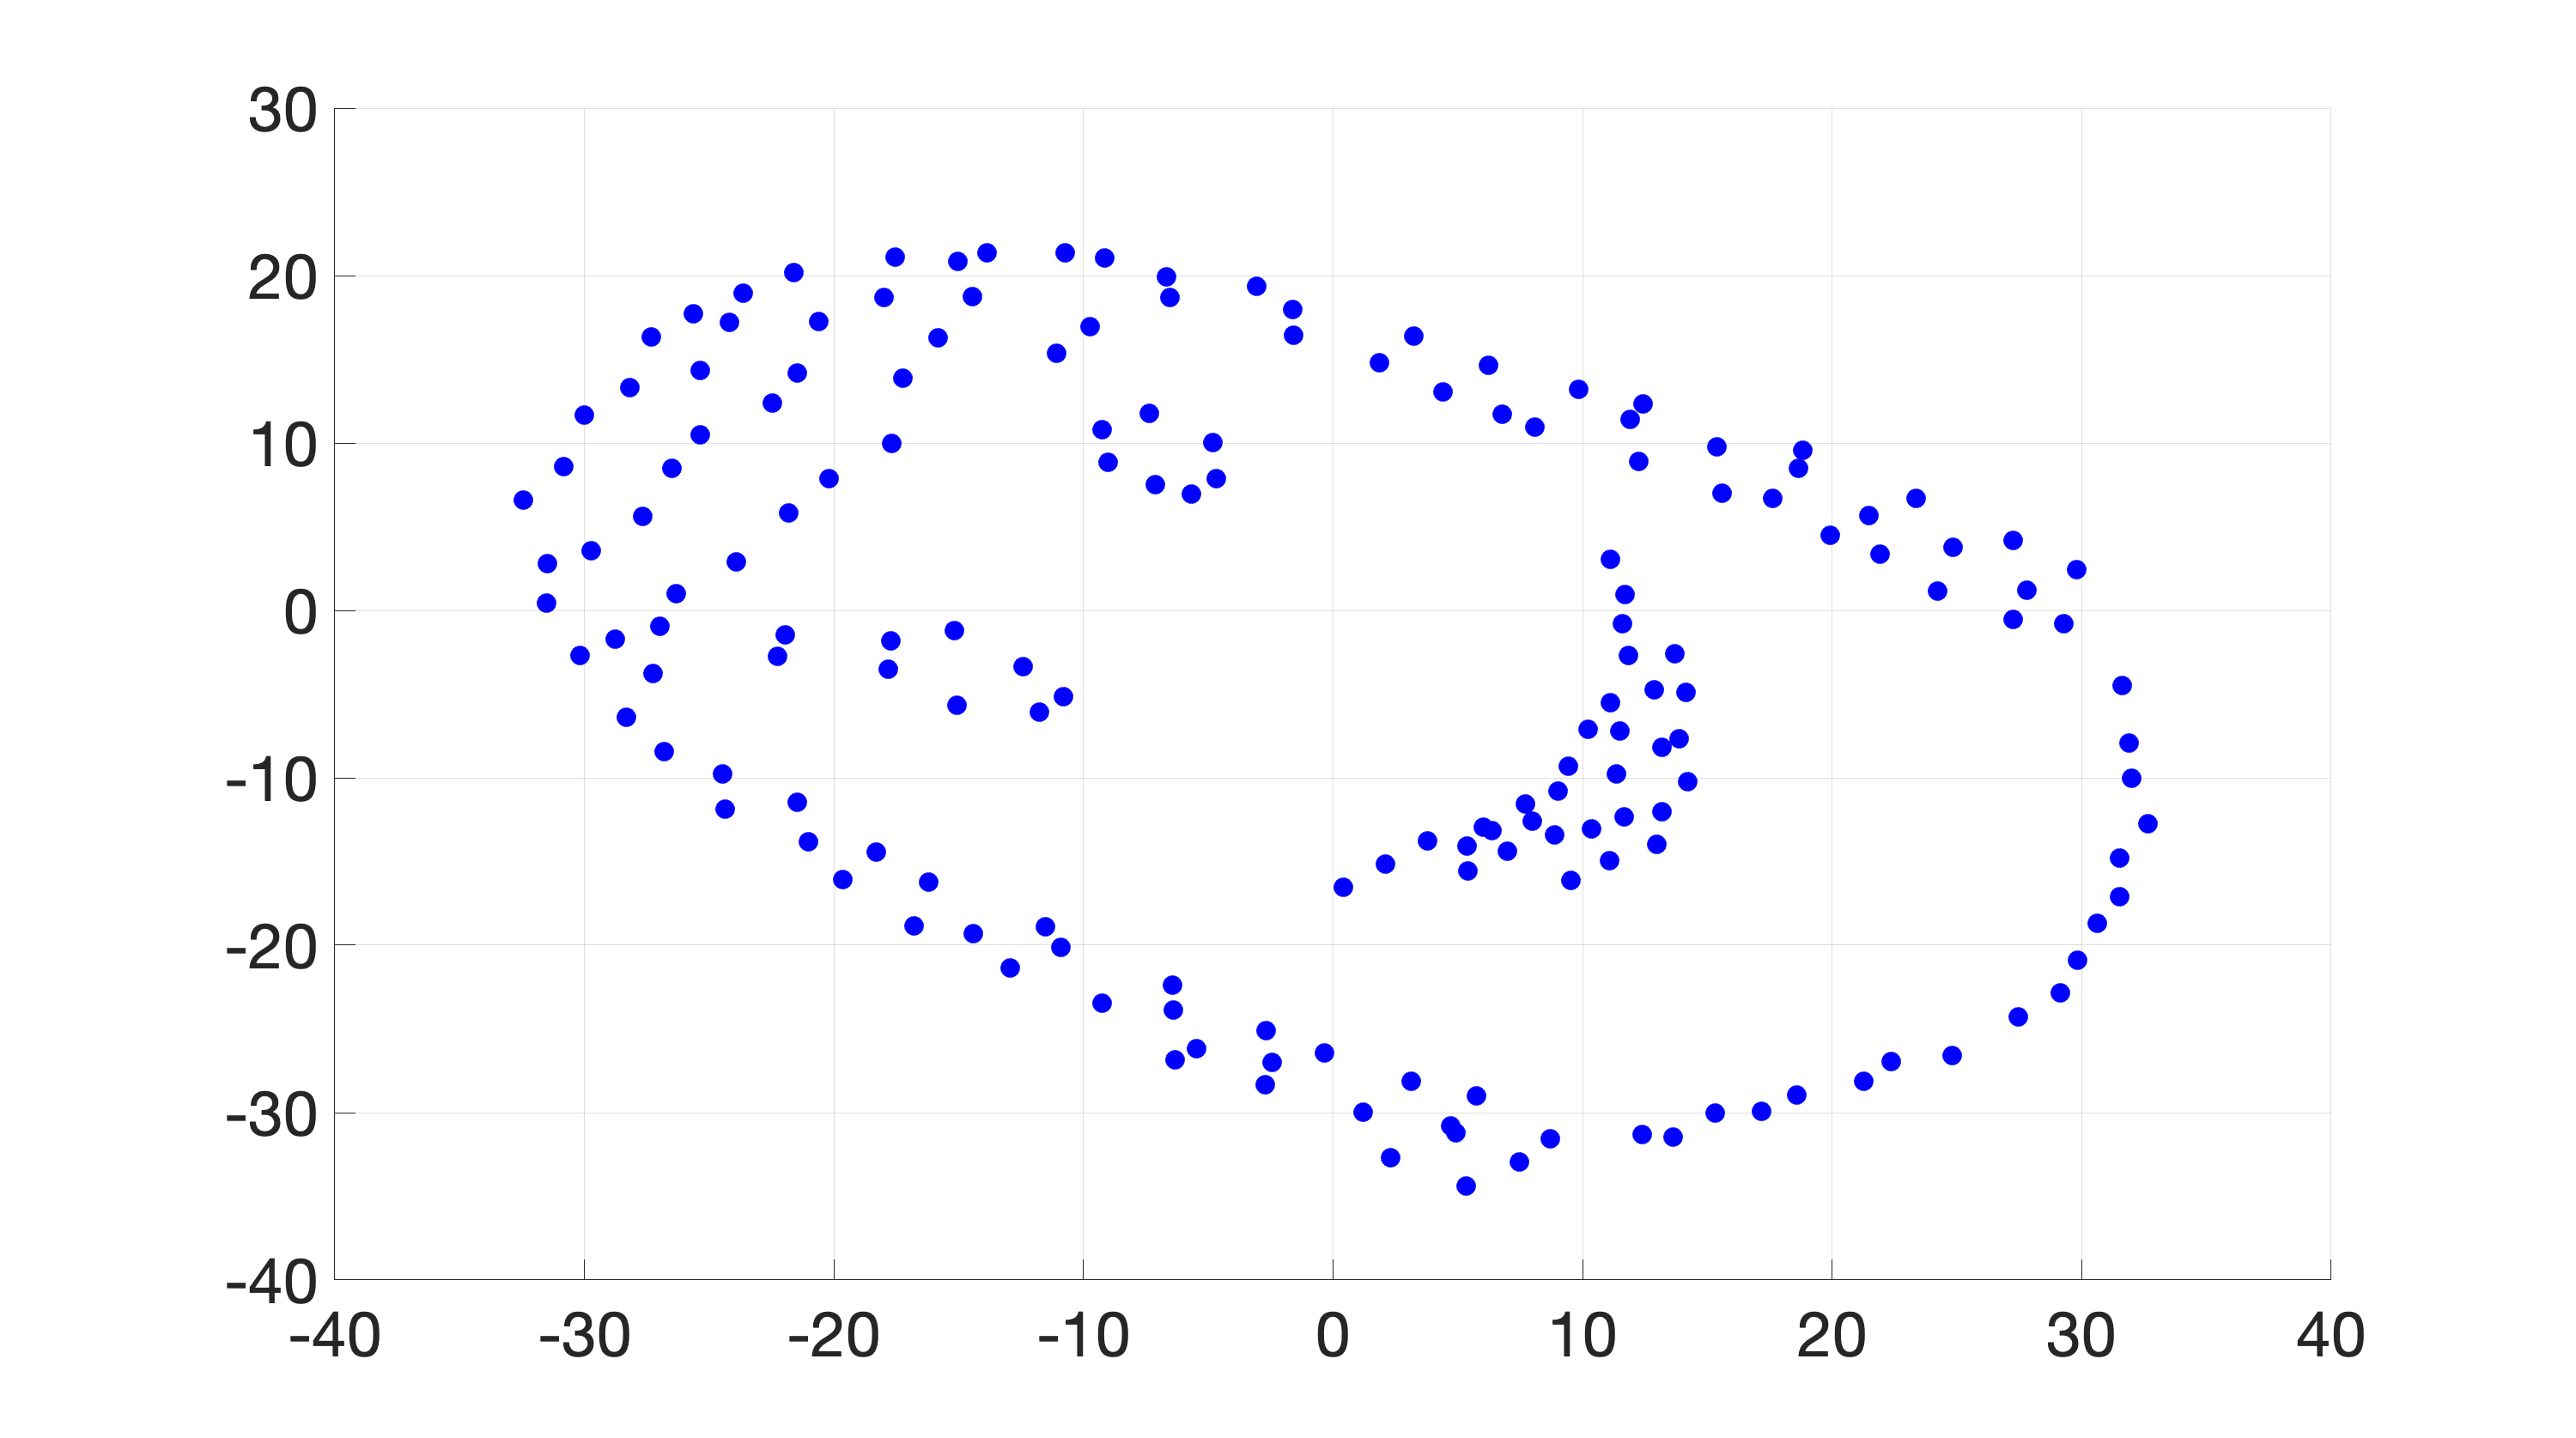
\includegraphics[width=0.9\textwidth]{figures/task4_sol.png}
	\caption{Best solution to the optimization problem using the LM algorithm for the dataset of task 4 and $k=2$, obtaining $f(\mathbf{y}_{sol}) = 7.6430\times 10^{-5}$.}
	\label{fig:task4_sol}
\end{figure}
%\mathbf{y} = \mathrm{col}(\mathbf{y_1},\ldots,\mathbf{y_N}) \quad  \text{and} \quad
It is now important to analyze the uniqueness of the solutions. In fact consider
\begin{equation*}\label{key}
 \bar{\mathbf{y}} = \mathrm{col}(\mathcal{T}\mathbf{y_1}+\mathbf{w},\ldots,\mathcal{T}\mathbf{y_N}+\mathbf{w})\:,
\end{equation*}
where $\mathcal{T} \in \mathbb{R}^{k\times k}$ is a rotation matrix and $\mathbf{w}\in\mathbb{R}^{k}$. It is easily verified that 
\begin{equation*}\label{key}
||\mathbf{\bar{y}_m}-{\mathbf{\bar{y}_n}}|| = ||\mathbf{y_m}-\mathbf{y_n}||
\end{equation*}
for every pair $(m,n):m \in \{1,\ldots,N\}, n \in \{1,\ldots,N\}$. Therefore
\begin{equation*}\label{key}
f(\mathbf{\bar{y}}) = f(\mathbf{y})\:.
\end{equation*}
It is, then, evident that if a global minimum is found, there are infinitely many other global minimums obtained via a rotation and translation of every $\mathbf{y_i}, \; i \in \{1,\ldots,N\}$. For this reason the previously shown solution, conjectured to be an estimate of a global solution, is not unique. In fact, analyzing the solution of the second best solution found, out of the $24$ computation, shown in Fig. \ref{fig:task4_sol_2}. In fact, even though both solutions achieve the same objective function value $f(\mathbf{y}_{sol}) = 7.6430\times 10^{-5}$, they are the result of a rotation and translation of each other. 
\begin{figure}[ht!]
	\centering
	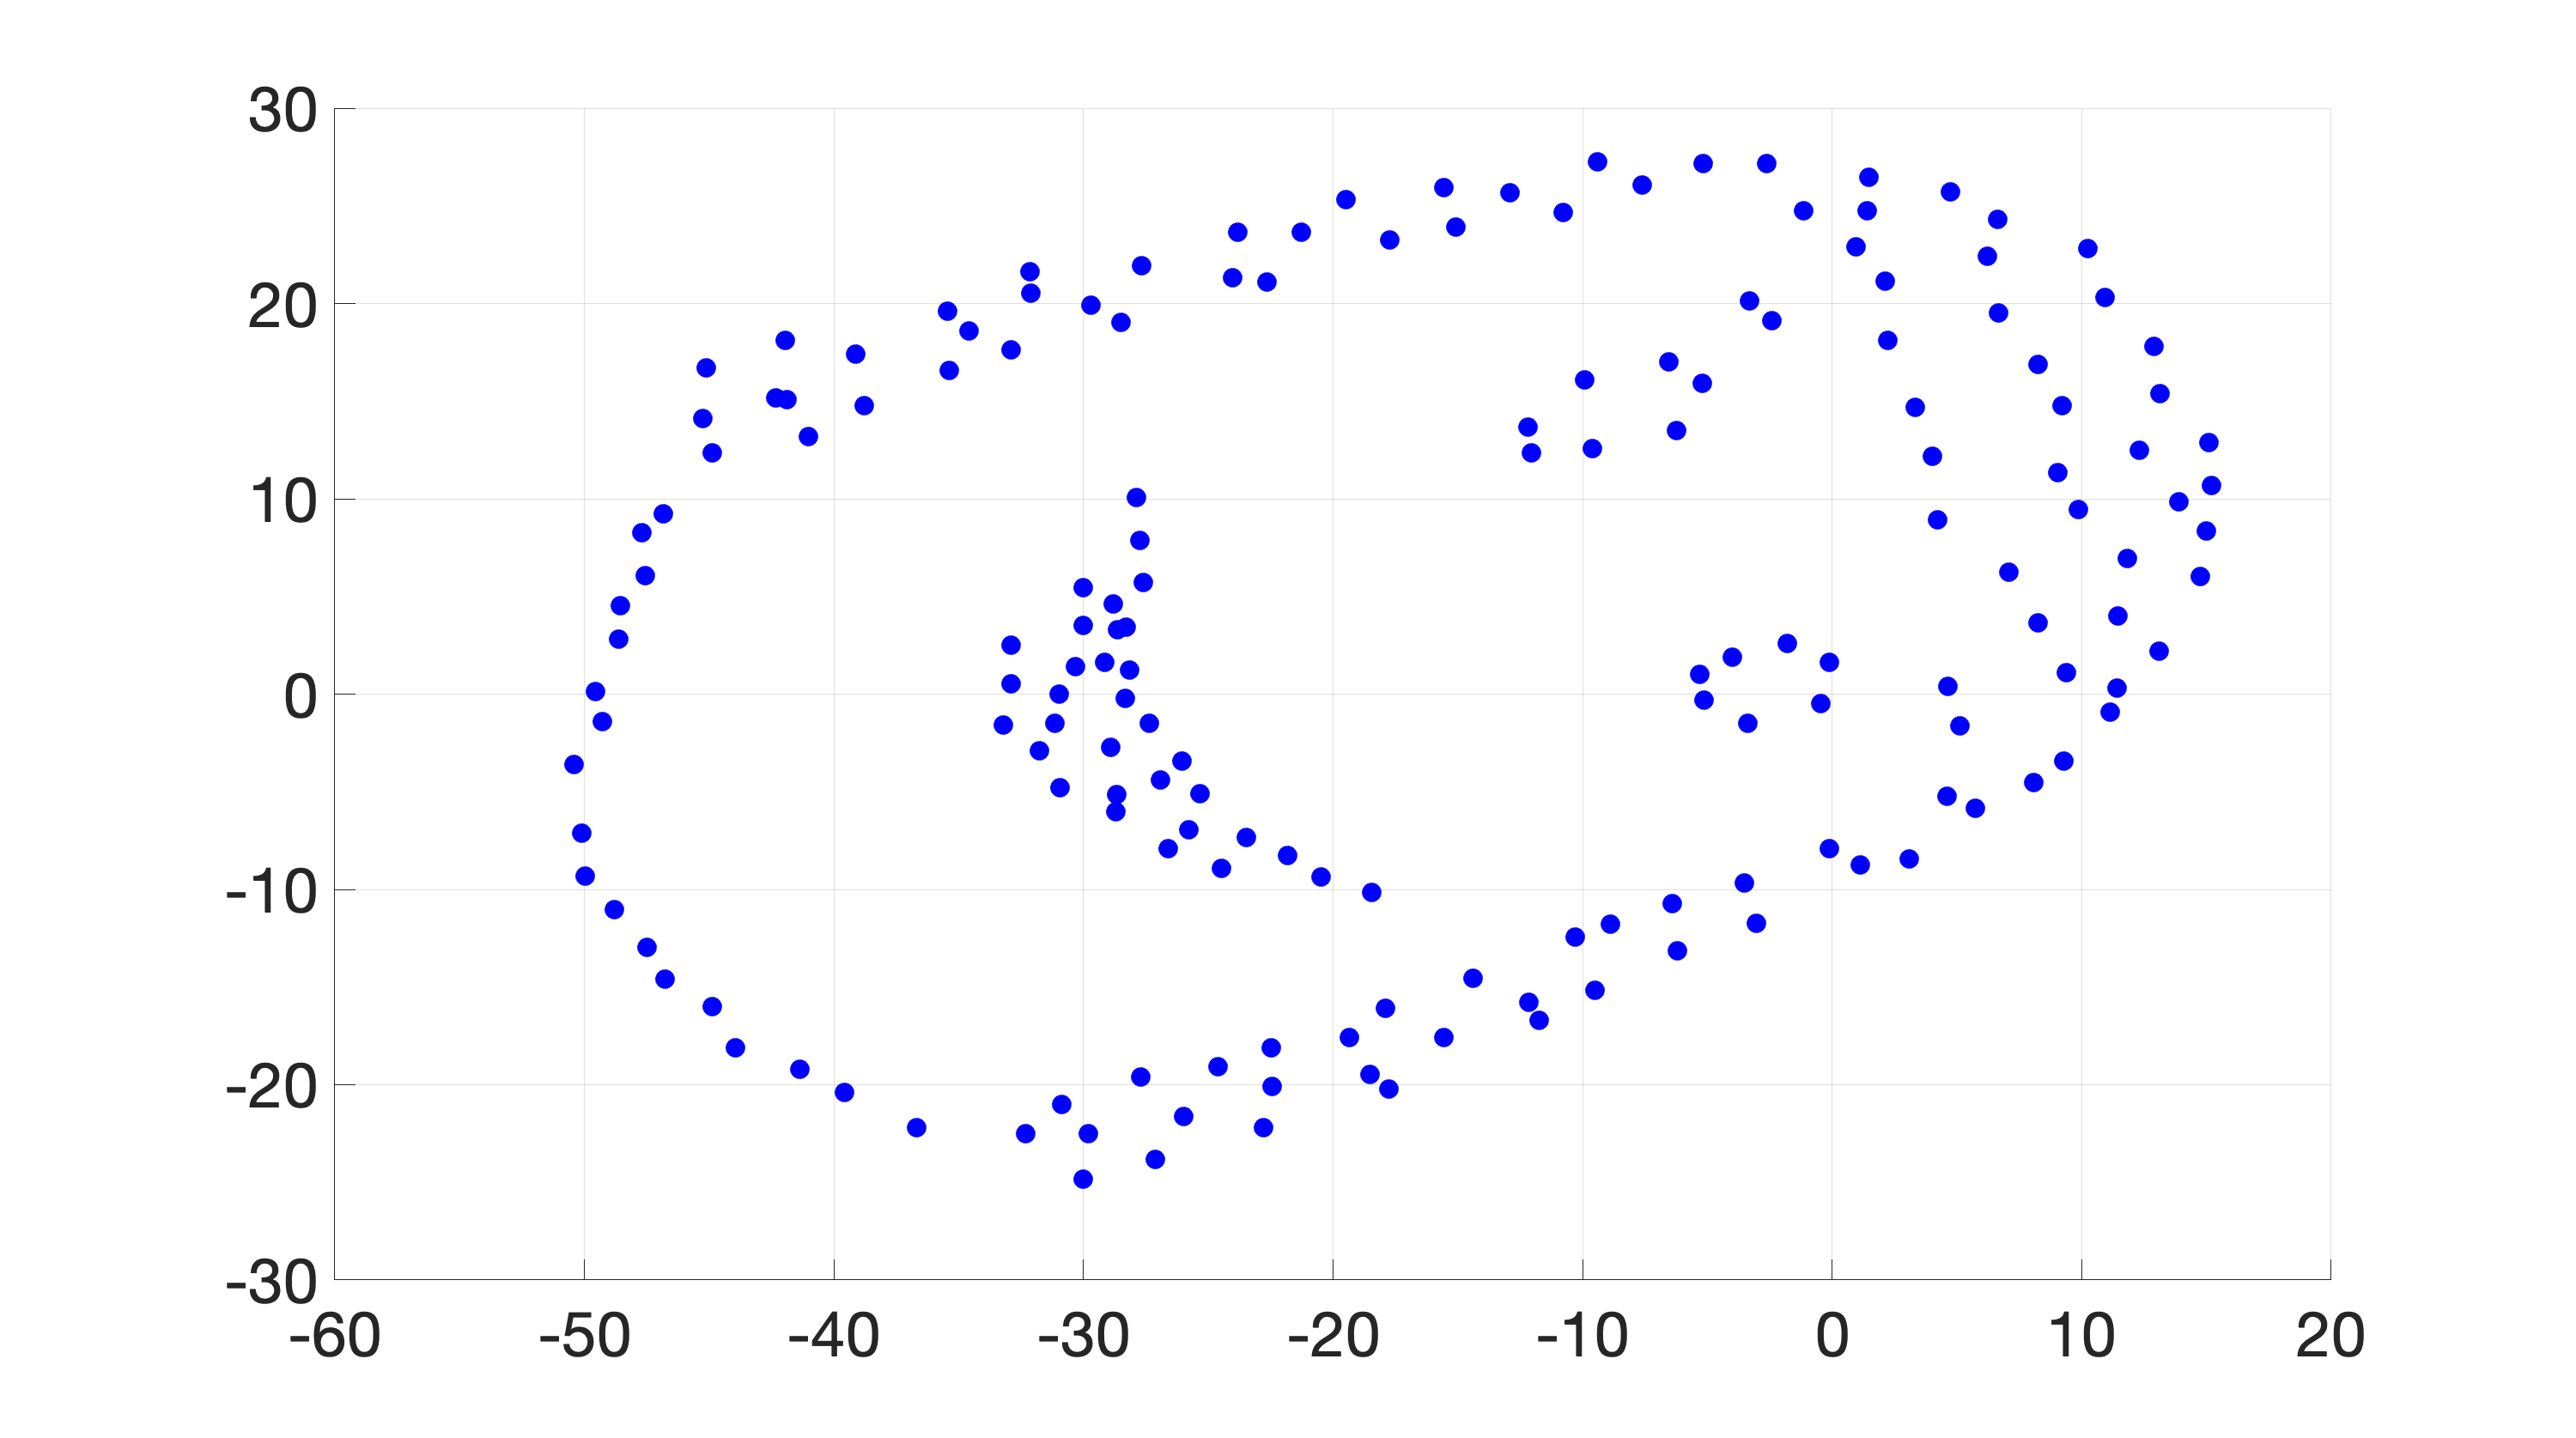
\includegraphics[width=0.9\textwidth]{figures/task4_sol_2.png}
	\caption{Second best solution to the optimization problem using the LM algorithm for the dataset of task 4 and $k=2$, obtaining $f(\mathbf{y}_{sol}) = 7.6430\times 10^{-5}$.}
	\label{fig:task4_sol_2}
\end{figure}

The following question now arises naturally: if the additional degrees of freedom (d.o.f.) of the rotation ($k-1$ d.o.f.) and of the translation ($k$ d.o.f) are suppressed, constraining the optimization problem, is a solution obtained unique? First, the optimization problem can be constrained imposing 
\begin{equation*}\label{key}
\mathbf{y_1} = \mathbf{0}_{k\times 1} \quad \text{and}  \quad  \mathbf{y_2} = \alpha\mathrm{col}(1,\mathbf{0}_{(k-1)\times 1})\:,
\end{equation*} 
with $\alpha \in \mathbb{R}$. The optimization problem becomes 
\begin{equation}\label{eq:problemModifiedT4}
\begin{array}[t]{ll} 
\underset{(\alpha,\mathbf{y_3},\ldots,\mathbf{y_N}) \in \mathbb{R} \times \mathbf{R}^{k}\times \ldots \times \mathbf{R}^{k} }{\text{minimize}} & (\alpha-D_{1,2})^2+\sum_{n=3}^{N}\left(||\mathbf{y_n}||_2-D_{mn}\right)^2\\
&+ \sum_{n=3}^{N}\left(||\alpha\mathrm{col}(1,\mathbf{0}_{(k-1)\times 1})-\mathbf{y_n}||_2-D_{mn}\right)^2\\
&\\
& +\sum_{m=3}^{N}\sum_{n=m+1}^{N}\left(||\mathbf{y_m}-\mathbf{y_n}||_2-D_{mn}\right)^2
\end{array}\:,
\end{equation}
with 
$\mathbf{y} = \mathrm{col}\left(\mathbf{0}_{k\times 1},\alpha\mathrm{col}(1,\mathbf{0}_{(k-1)\times 1}),\mathbf{y_3} \ldots,\mathbf{y_N}\right) \in \mathbb{R}^{Nk}$, which is still nonconvex. In fact, it is easily proven that if a global solution is found, it is not necessarily unique. As a matter of fact, considering 
\begin{equation*}\label{key}
\mathbf{D} = \begin{bmatrix}
0 & 4 & \sqrt{5} \\ 4 & 0 & 5 \\ \sqrt{5} & 5 & 0 
\end{bmatrix}
\end{equation*} 
both 
\begin{equation*}\label{key}
\mathbf{y} = \begin{bmatrix}
0 \\ 0 \\ 4 \\ 0 \\ 1 \\ 4 
\end{bmatrix}\quad \text{and} \quad \mathbf{y} = \begin{bmatrix}
0 \\ 0 \\ 4 \\ 0 \\ 1 \\ -4 
\end{bmatrix}
\end{equation*}
are solutions to \eqref{eq:problemModifiedT4}, with $f(\mathbf{y})=0$. Notice that can not be obtained from each other via a rotation and translation. Therefore, even if the additional $2k-1$ degrees of freedom of the solutions to the original problem \eqref{eq:problemT4} are suppressed, there is no guarantee that if a global solution is found, it is unique. In fact, inspired by this example it is not difficult to notice that if every $\mathbf{y_m}$ is reflected on the axis corresponding to the first coordinate, then the objective function value remains unchanged. Even if this d.o.f. is suppressed via an additional constraint, we could not find any uniqueness guarantees. 

In conclusion, given the thorough analysis conducted, the solution found is not unique. In fact, infinitely many solutions can be found via a translation, rotation, and/or reflection on the axis corresponding to the first coordinate.
%To suppress this additional d.o.f. the following constraint would have to be imposed to \eqref{eq:problemModifiedT4}
%\begin{equation}\label{key}
%\mathrm{card}\{n:[0\;1\;0\;\ldots\;0]\mathbf{y_n} \geq 0\;,n \in \{3,\ldots,N\}\} \geq 1 \;,
%\end{equation}  
%\textit{i.e.}, at least one $y$

\end{document}